\section{Mediciones}

Para las mediciones, creamos subconjuntos de dos tipos distintos. Uno que lo llamamos \textit{jugadores} y otro que lo llamamos \textit{abecedario}.
El primero contiene una lista con subconjuntos de jugadores de fútbol argentino, mientras que el segundo contiene una lista con subconjuntos de combinaciones de letras del abecedario. Esto debido a que queríamos obtener comportamientos menos repetitivos, ya que tenemos un máximo de 43 jugadores distintos, mientras que el abecedario tiene 26 letras, y en base a ellas, podemos hacer combinaciones de letras para generar "palabras" de distintos tamaños, los cuales se repetiran en menor medida.
Con ello conseguimos obtener resultados más amplios (no es lo mismo un conjunto de 1 millón de elementos distintos con una solución de Hitting Set hasta de 43 elementos, a una solución con 1 millón de elementos distintos).

Además, notamos que los procesos de fondo del sistema nos generaba distorciones en los tiempos de ejecución de una misma muestra. Resolvimos este problema
realizando varias mediciones para el mismo escenario de subconjuntos y tomando el promedio de los tiempos obtenidos. Esta estrategia nos permitió abordar otro problema significativo: el orden en el que se evalúan los jugadores en cada subconjunto adquiere una importancia relevante en el rendimiento final del algoritmo. Esto depende especialmente de la frecuencia con la que cada jugador aparece en los demás subconjuntos. 

Asimismo, al definir arbitrariamente cada escenario, puede ocurrir que en una cantidad 
$x$ de subconjuntos, los jugadores incluidos en cada uno sean considerablemente diferentes o poco comunes, lo que representa un caso desfavorable. En contraste, en una cantidad de conjuntos $x+1$, podría darse una situación mucho más favorable, con una mayor similitud entre los jugadores incluidos en cada conjunto. Esto puede llevar a una diferencia significativa en los tiempos de ejecución, a pesar de que la cantidad de conjuntos varíe en una sola unidad.

Siguiendo las estrategias explicadas, realizamos mediciones variando solamente la cantidad de subconjutos y comparando el tiempo de ejecución de los diferentes algorítmos analizados a lo largo del informe: Backtracking, algorítmo Greedy Máximo por grupo, algorítmo Greedy Máximo global con recálculo, Programación Lineal Entera y Programación Lineal Continua.

Al evaluar los algoritmos con orden teórico exponencial, Backtracking y Programación Lineal Entera, podemos corroborar a través de los gráficos una clara tendencia al aumento significativo en el tiempo de ejecución conforme se incrementa la cantidad de subconjuntos, en comparación con otros algoritmos, especialmente los que emplean el método Greedy.

La gráfica de nuestra implementación de Backtracking confirma su comportamiento exponencial, concordando con su cota teórica. Por otro lado, el algoritmo de Programación Lineal Entera, contrario a lo esperado, presenta una gráfica más cercana a una función lineal, asemejandose en tiempo de ejecución con el algorítmo de Programación Lineal Continua. Esto se debe a las optimizaciones implementadas en la librería $pulp$ utilizada para su ejecución, las cuales reducen significativamente su tiempo de ejecución en comparación con su complejidad teórica. Es importante mencionar que la visualización de una curva exponencial en este algoritmo solo ocurre en situaciones donde las optimizaciones no influyen de manera considerable.

Por otro lado, podemos observar que la curva de Programación Lineal Continua se asemeja a una curva polinómica. De esta manera, mediante el gráfico y la validación a través del error cuadrático medio, hemos comprobado que la curva de un polinomio de grado 9?? se adapta de manera más precisa a nuestros datos, corroborando la cota teórica. De esta forma pudimos comprobar empíricamente que la complejidad tiende a $\operatorname{O}(n^{9})$. 

En el siguiente gráfico, se ilustra el grado de aproximación, variando $b$ (Figura 1) y manteniendola constante (Figura 2). Para poder corroborar nuestra cota máxima de aproximación, hicimos variar este parámetro $b$ en un intervalo desde $[25:30]$. Como en la gráfica se puede observar que la peor aproximación es $NUM_MAX$, luego se comprueba que la cota máxima es efectivamente en cada escenario es $b-1$.

Por otra partem al examinar los algoritmos que emplean la estrategia de diseño Greedy, ambos siguen una tendencia polinomial. En el primer gráfico, se observa que el RMSE presenta un menor valor en la regresión lineal. Esto se debe a que la variable $b$ permanece constante para cada escenario, variando únicamente la cantidad de subconjuntos ($m$). En contraste, al aumentar la variable $b$ a medida que se aumenta la cantidad de subconjuntos, se puede visualizar su tendencia polinómica no lineal, evidenciando la cota teórica. 

Asimismo, se destaca una marcada diferencia en los tiempos de ejecución entre el algoritmo Greedy Máximo por grupo y el algoritmo Greedy Máximo global. El primero muestra una ejecución significativamente más rápida en todos los escenarios comparado con el segundo. Sin embargo, al analizar las soluciones obtenidas, se evidencia que el algoritmo Greedy Máximo global se acerca más a la solución óptima en todos los casos estudiados.

Esta divergencia plantea una dificultad al momento de decidir cuál enfoque es más adecuado. Por un lado, el algoritmo por grupo se destaca por su eficiencia temporal, ofreciendo tiempos de ejecución notoriamente inferiores y, por otro lado, el enfoque global muestra una mayor aproximación a la solución óptima.

!!! INSERTAR GRAFICOS !!!

% \begin{figure}[H]
%     \centering
%     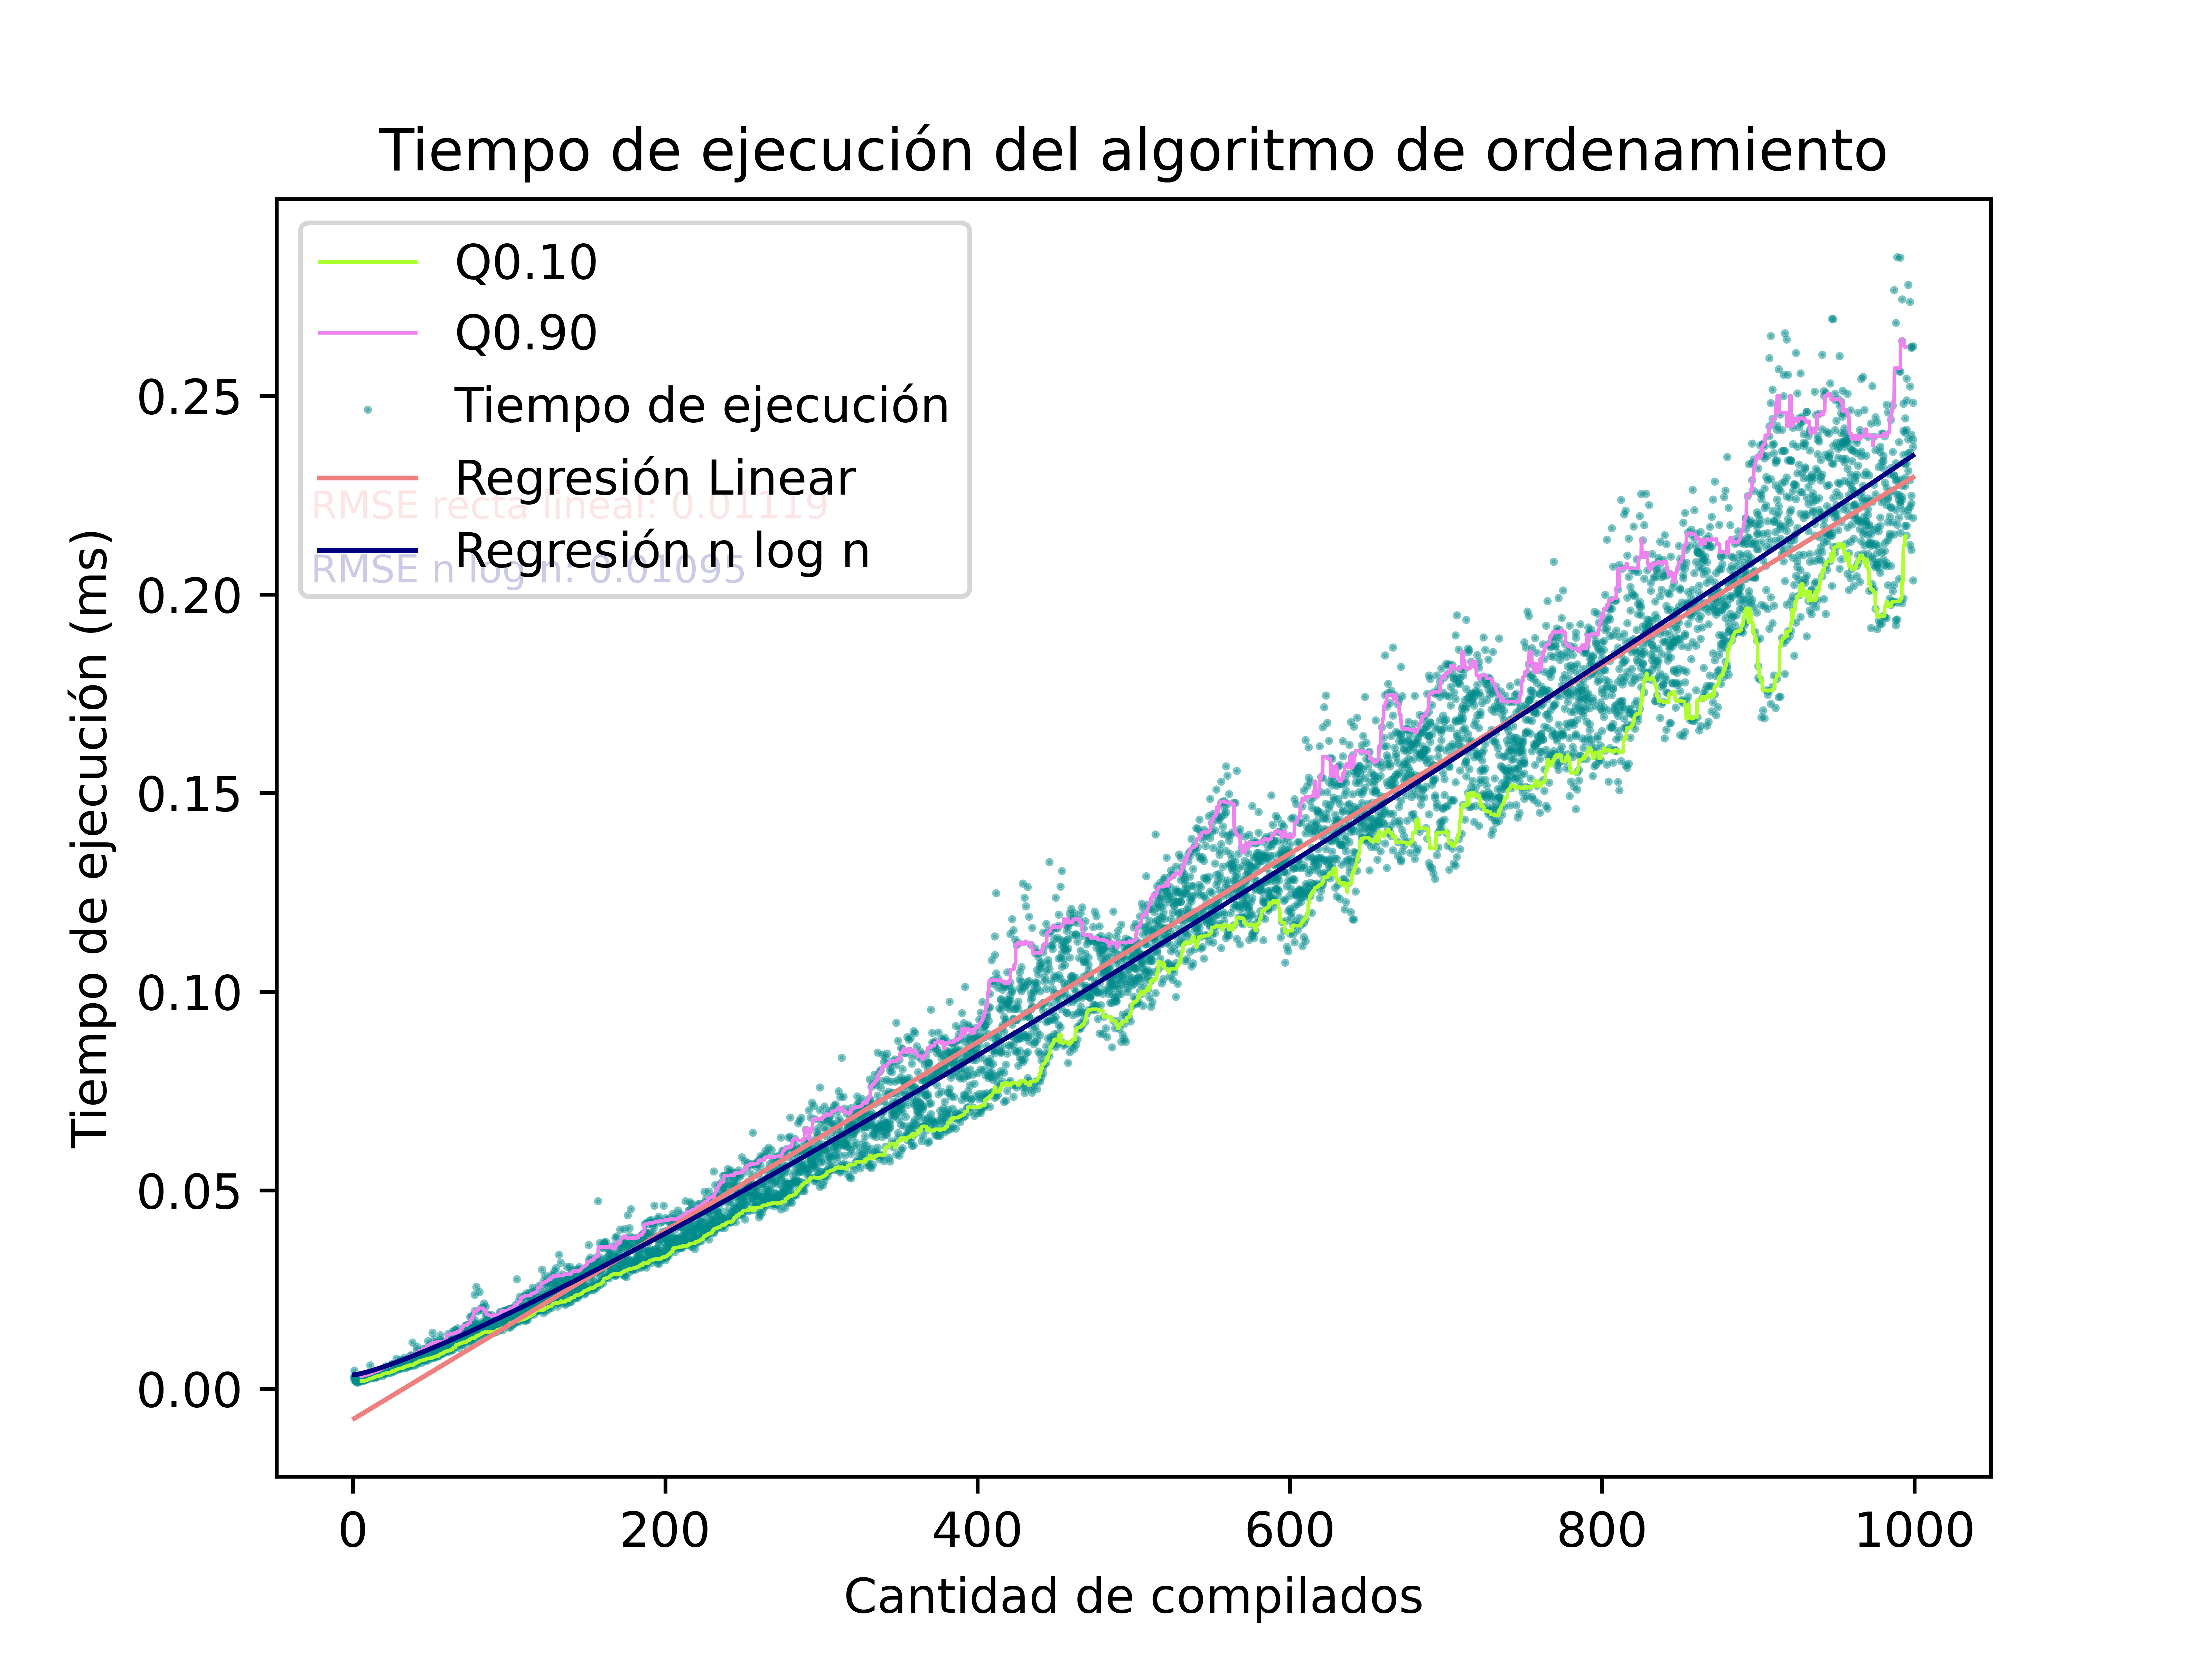
\includegraphics[width=0.8\textwidth]{img/tiempos_valores_bajos_puntos.png}
%     \caption{Tendencia de la complejidad algoritmica para $n$ pequeños.}
%     \label{fig:tiempos_valores_bajos_puntos}
% \end{figure}

% \begin{figure}[H]
%     \centering
%     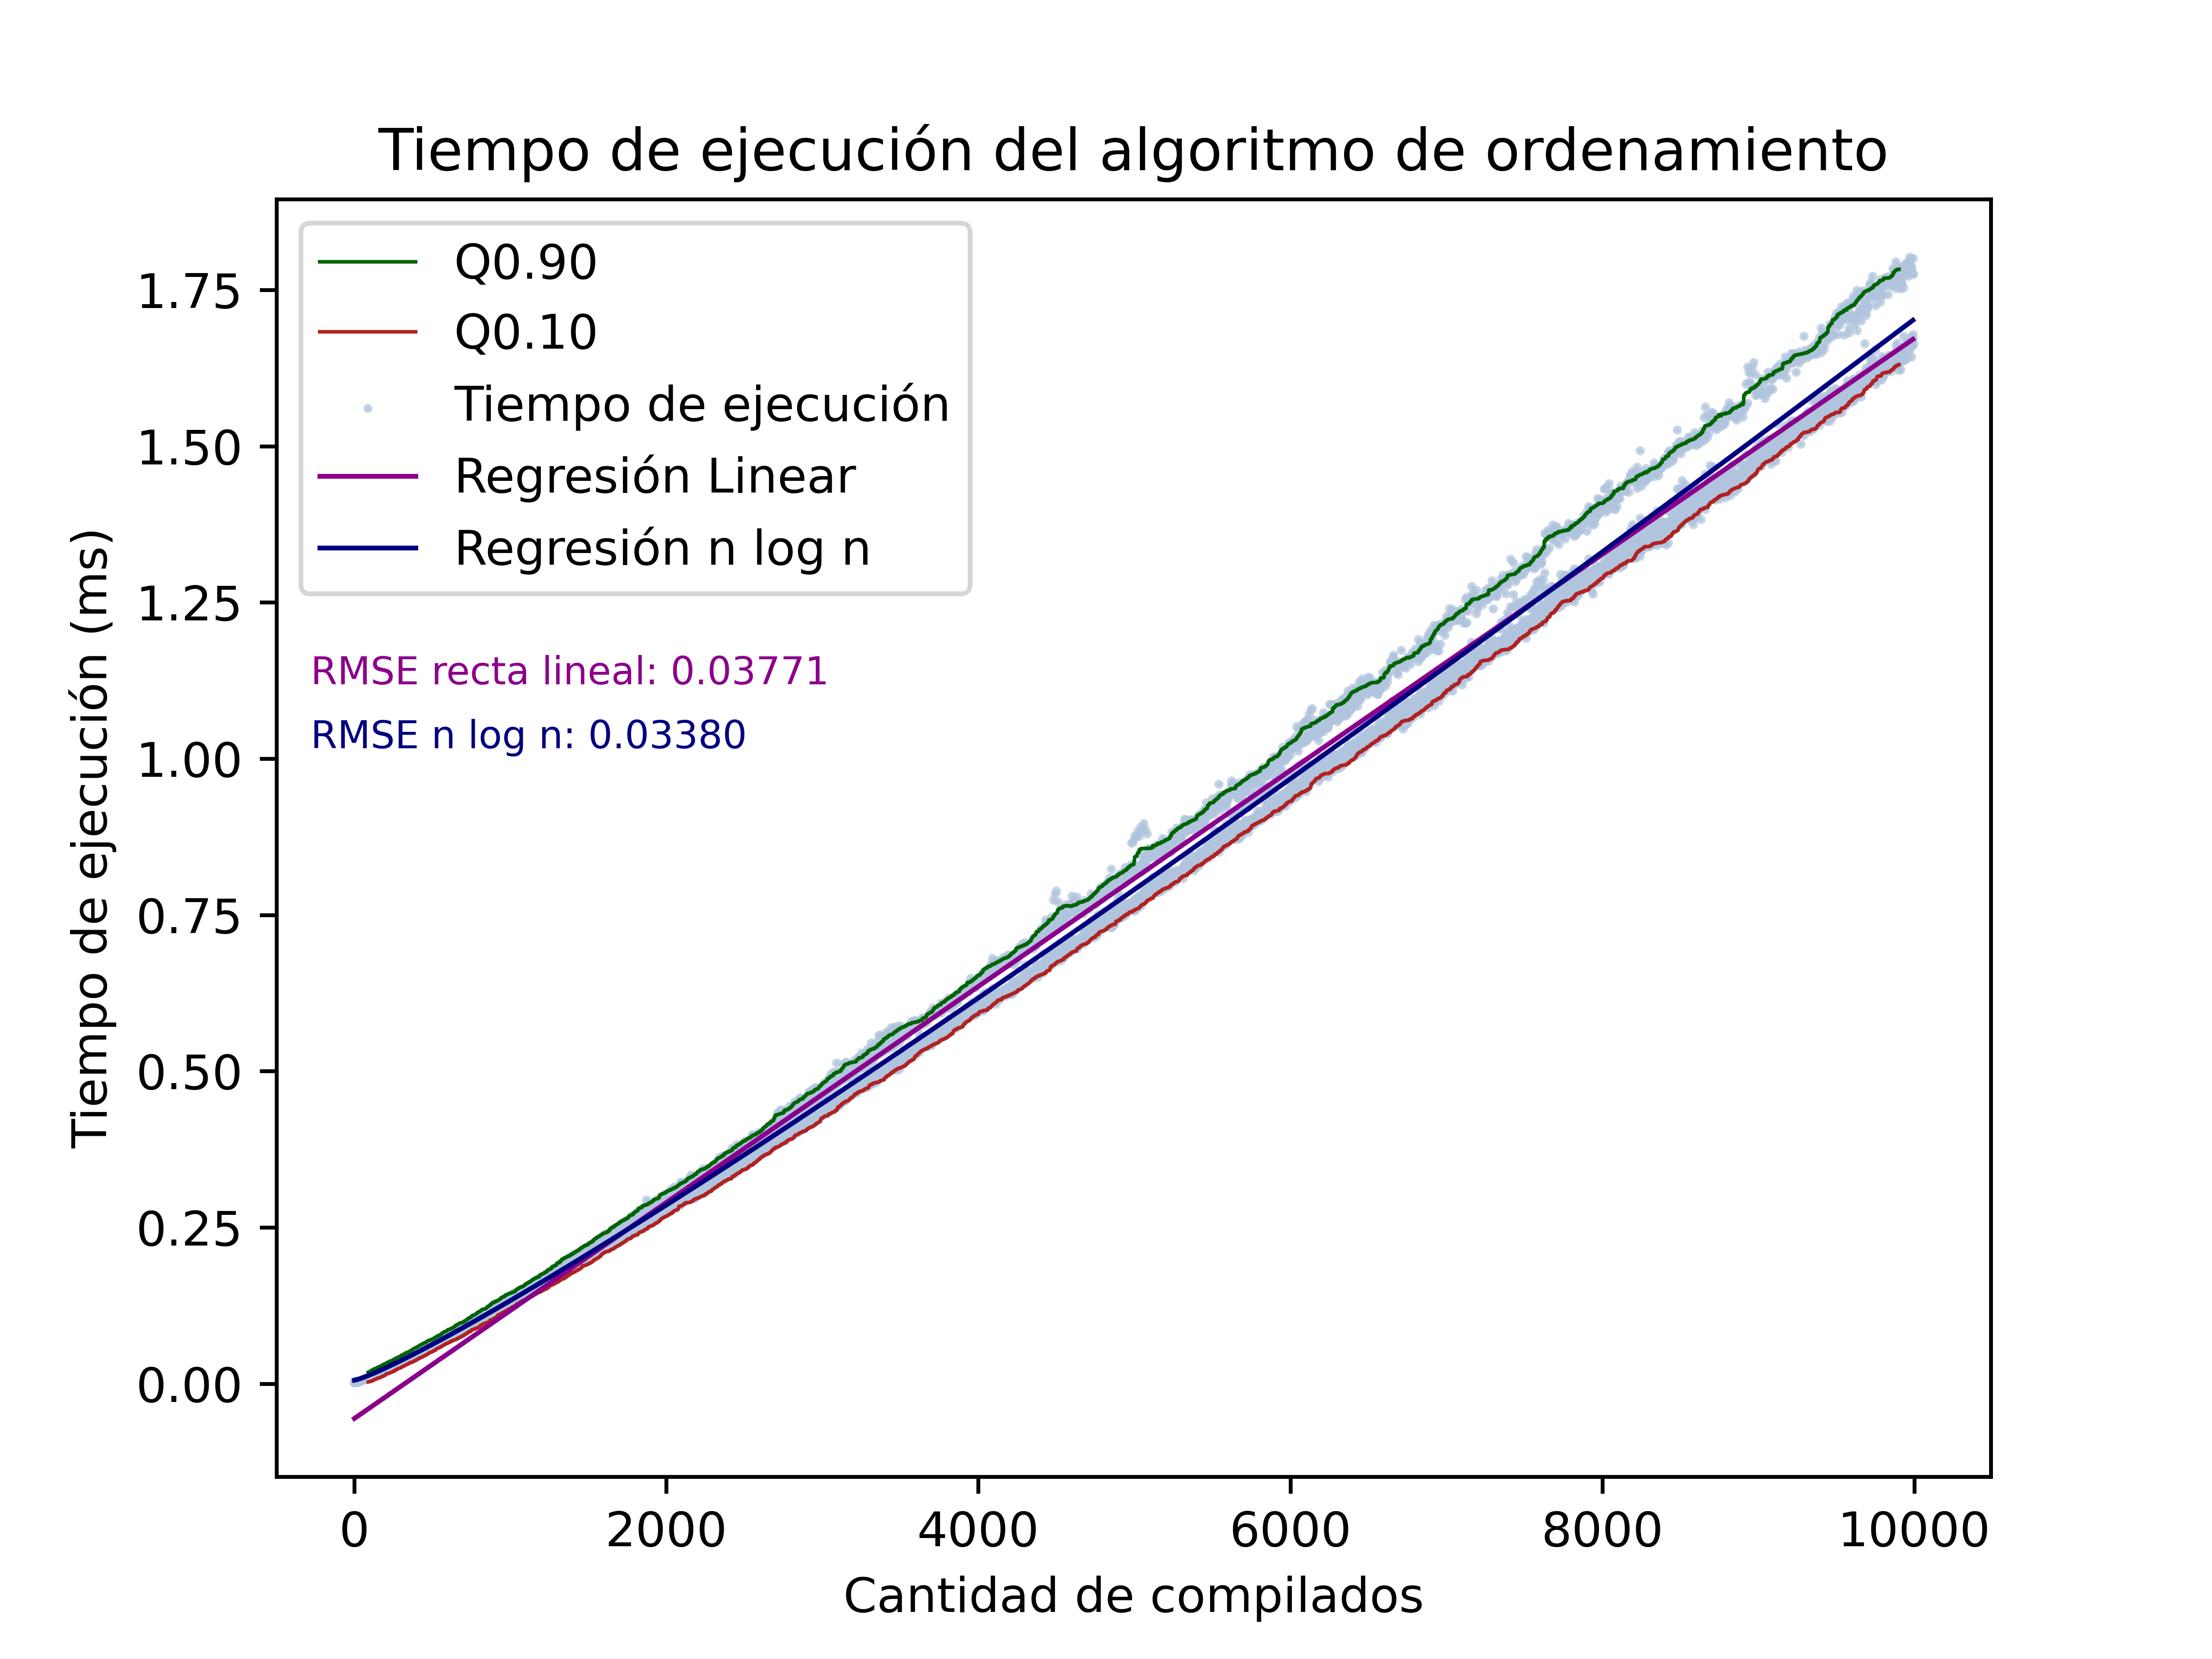
\includegraphics[width=0.8\textwidth]{img/tiempos_valores_altos_puntos.png}
%     \caption{Tendencia de la complejidad algoritmica para $n$ grandes.}
%     \label{fig:tiempos_valores_altos_puntos}
% \end{figure}
